\documentclass{beamer}

\usefonttheme{professionalfonts} % using non standard fonts for beamer
\usefonttheme{serif} % default family is serif

%\usepackage{hyperref}

%\usepackage{minted}

\usepackage{animate}

\usepackage{graphicx}

\def\Put(#1,#2)#3{\leavevmode\makebox(0,0){\put(#1,#2){#3}}}

\usepackage{color}

\usepackage{tikz}

\usepackage{amssymb}

\usepackage{enumerate}


\newcommand\blfootnote[1]{%

  \begingroup

  \renewcommand\thefootnote{}\footnote{#1}%

  \addtocounter{footnote}{-1}%

  \endgroup

}

\makeatletter

%%%%%%%%%%%%%%%%%%%%%%%%%%%%%% Textclass specific LaTeX commands.

 % this default might be overridden by plain title style

 \newcommand\makebeamertitle{\frame{\maketitle}}%

 % (ERT) argument for the TOC

 \AtBeginDocument{%

   \let\origtableofcontents=\tableofcontents

   \def\tableofcontents{\@ifnextchar[{\origtableofcontents}{\gobbletableofcontents}}

   \def\gobbletableofcontents#1{\origtableofcontents}

 }

%%%%%%%%%%%%%%%%%%%%%%%%%%%%%% User specified LaTeX commands.

\usetheme{Malmoe}

% or ...

\useoutertheme{infolines}

\addtobeamertemplate{headline}{}{\vskip2pt}



\setbeamercovered{transparent}

% or whatever (possibly just delete it)

\makeatother

\begin{document}
\title[DCEL report]{RIDIR Report}
\author[AC]{Andres Calderon}
\institute[Winter'20]{University of California, Riverside}
\makebeamertitle
\newif\iflattersubsect

\AtBeginSection[] {
    \begin{frame}<beamer>
    \frametitle{Outline} 
    \tableofcontents[currentsection]  
    \end{frame}
    \lattersubsectfalse
}

\AtBeginSubsection[] {
    \begin{frame}<beamer>
    \frametitle{Outline} 
    \tableofcontents[currentsubsection]  
    \end{frame}
}

\begin{frame}{Fixing previous bugs...}
    \begin{itemize}
     \item There were related with the current precision on float-point operations.  Currently set at 4 digits.
    \end{itemize}
    \centering
	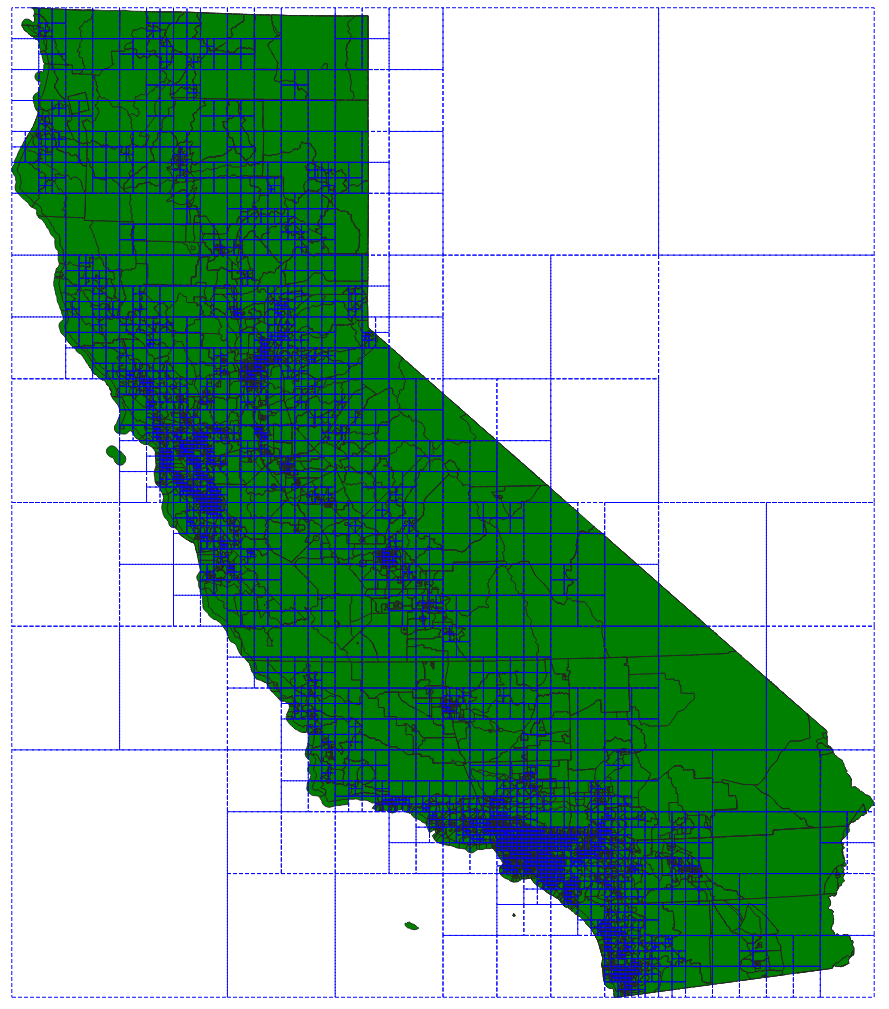
\includegraphics[trim=1cm 0 1cm 0, clip, width=0.45\textwidth]{figures/DCEL}
\end{frame}

\begin{frame}{Some statistics...}
    \centering
    \begin{tabular}{ll}
        \hline
        \textbf{Phase} & \textbf{Execution time [s]} \\
        \hline
        Partitioning & 10.22 \\
        Building single DCELs & 4.02 \\
        Updating empy cells & 7.82 \\
        Merging DCELs & 5.28 \\
        Checking single-label faces & 4.34 \\
        \textbf{Total} & \textbf{31.69} \\
        \hline
    \end{tabular}
\end{frame}

\begin{frame}{Exploring sequential implementation...}
    \begin{itemize}
     \item CGAL 5.0.2 - 2D Arrangements\footnote{\tiny Available at \url{https://doc.cgal.org/latest/Arrangement_on_surface_2/index.html}}
    \end{itemize}
    \centering
	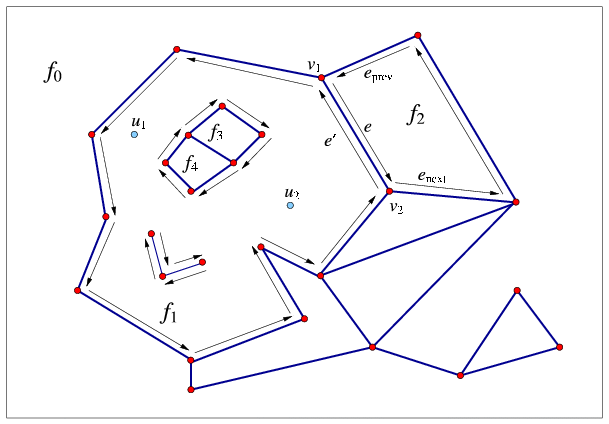
\includegraphics[trim=1cm 0 1cm 0, clip, width=0.6\textwidth]{figures/CGAL}
\end{frame}

\begin{frame}{What's next?}
    \begin{itemize}
        \item Integrating overlay operators...
        \item Cleaning and Validation...
        \item Tuning cluster parameters...
        \item Benchmarking with sequential tool...
    \end{itemize}
\end{frame}

\end{document}
